% Speaker script for slides.tex (short version; the script of ../notes.tex with
% references to panels removed from the slides adjusted).  Build: ./build.sh
% build_html.py converts this file into notes.html and into the notes panel of
% slides.html, so keep to the macros used here (\slidenote, \emph, \textbf,
% inline $...$ with the symbols listed in build_html.MATH, ^{} and _{}).
% Everything from the first slide note up to the first new-page command is
% parsed; the backup part is separated with a clear-page command so that it
% stays in that range.
\documentclass[12pt,a4paper]{article}
\usepackage[T1]{fontenc}
\usepackage[utf8]{inputenc}
\usepackage{lmodern}
\usepackage[a4paper,margin=2.0cm]{geometry}
\usepackage{graphicx}
\usepackage{xcolor}
\usepackage{enumitem}
\usepackage[colorlinks=true,urlcolor=blue!55!black]{hyperref}
\definecolor{accent}{HTML}{1F5FA8}
\definecolor{muted}{HTML}{6B7280}
\setlength{\parindent}{0pt}
\setlength{\parskip}{6pt}
\linespread{1.12}

% \slidenote{page in slides.pdf}{label shown}{title}{timing}
\newcommand{\slidenote}[4]{%
  \par\bigskip\noindent
  \begin{minipage}[t]{.3\textwidth}\vspace{0pt}
    \includegraphics[page=#1,width=\linewidth]{slides.pdf}
  \end{minipage}\hfill
  \begin{minipage}[t]{.66\textwidth}\vspace{0pt}
    {\large\bfseries\color{accent}#2.\ #3}\par
    {\small\color{muted}#4}
  \end{minipage}\par\smallskip}

\begin{document}

{\LARGE\bfseries Speaker script\par}
\smallskip
{\large Extremality shift of rotating black holes at finite Gauss--Bonnet coupling\par}
{\color{muted}Five minutes, five slides plus a closing one: about 650 words at a calm pace. The times are targets; the elapsed time is in brackets. Paragraphs marked ``Background'' are for you, not part of the script. Slides A1--A5 are backup for questions and are not part of the five minutes; their notes explain the method and the physics in more detail.\par}

\slidenote{1}{1}{Title}{0:15 \quad [0:15]}

This is joint work by Cecilia Bejarano, David Blanco, Guillem Pérez-Nadal and
myself. Most of the code, the computations and the writing were done by two AI
agents, Claude Code and Codex, under our direction.

\slidenote{2}{2}{Problem: the question}{1:05 \quad [1:20]}

A rotating black hole cannot spin arbitrarily fast for its mass. For Kerr the
bound is $J \le M^2$. When it is saturated the temperature drops to zero, and
the black hole is called \emph{extremal}.

In five dimensions with two equal angular momenta the bound reads: $M$ at least
three halves $\pi^{1/3} J^{2/3}$. That is the orange star.

This bound is a property of Einstein's equations. If we add the Gauss--Bonnet
term, the natural first higher-curvature correction, with a coupling $\alpha$,
the bound moves. How far? To first order in $\alpha$ the answer was known: the
extremal mass grows with slope exactly $\pi$, the dashed line. Our question was
what happens when $\alpha$ is \emph{not} small, that is, the question mark.

\textbf{Background: the action} (for you, not part of the timed script; use a
sentence of it if the audience needs it). In general relativity the dynamical
field is the metric $g_{\mu\nu}$. The Einstein--Hilbert action,
$\int \sqrt{-g}\,R$, with $R$ the Ricci scalar (the simplest scalar built from
the curvature), gives as Euler--Lagrange equations Einstein's equations,
$G_{\mu\nu} = 0$ in vacuum. They are second order in derivatives of the metric,
like Newton's or Maxwell's equations. The Gauss--Bonnet term,
$L_{\rm GB} = R^2 - 4R_{\mu\nu}R^{\mu\nu} + R_{\mu\nu\rho\sigma}R^{\mu\nu\rho\sigma}$,
is quadratic in the curvature, so it brings higher-derivative terms into the
action. Terms like this are expected for two reasons. In effective field theory,
general relativity is the first term of an expansion in curvature, and these are
the first corrections; their size is set by the coupling $\alpha$, which has
units of length squared. They also appear in the low-energy limit of string
theory. The Gauss--Bonnet combination is special in two ways: its field equations
stay second order, and in four dimensions it does not change the equations at all
(it is a total derivative). That is one reason to work in five dimensions.

\slidenote{3}{3}{Main result}{1:20 \quad [2:40]}

The key idea is thermodynamic. If we treat $\alpha$ as one more thermodynamic
variable, the first law gets a new term, $\Psi\,d\alpha$. At zero temperature
the $T\,dS$ term disappears, so at fixed spin $\Psi$ is exactly the slope we
want. We compute $\Psi$ on every numerical solution, 356 of them at 13
couplings, and extrapolate to zero temperature.

Here is the result: the slope against the scaled coupling
$y = \alpha/J^{2/3}$. At $y = 0$ we recover $\pi$, the green star. Then the slope
falls fast, to about 1.07, and rises again to 1.44 at the largest coupling we
reached. The open squares are an independent estimate from the mass curve.

Three messages. The slope is always positive, so Gauss--Bonnet makes the spin
bound tighter. It is far from constant, so the first-order formula fails
quickly. And it is not monotonic. The extremal mass itself (backup A3) grows by 31 percent, and the first-order line predicts a shift more than twice
as large as the real one.

\slidenote{4}{4}{Validation}{1:10 \quad [3:50]}

How do we know it is right? Three kinds of evidence.

First, known answers. Before computing anything new, the code reproduced a
published family of rotating Gauss--Bonnet black holes to two parts in ten
thousand. It also recovers the exact static solution and the value $\pi$ at
small coupling.

Second, independent routes. $\Psi$ can also be obtained from the Smarr relation,
using only the charges of a single solution, or as the integral of the
Gauss--Bonnet density outside the black hole. Neither uses our main method, and
both agree with it to about one part in a million. The bars show the worst
deviation of every check.

Third, the honest caveat. We never build a zero-temperature solution; we get
very cold and extrapolate. That extrapolation is the largest uncertainty, and it
is what the error bars in the result show.

\slidenote{5}{5}{Experience: what we learned}{1:05 \quad [4:55]}

Finally, what we learned about working with agents. The division of labour in the diagram worked well: we chose the question and kept doubting; Claude Code wrote
and ran the code; Codex acted as a referee and asked for checks. The referee
rounds mattered: one check a referee asked for actually \emph{failed} when it was
run. We compute the slope in two ways, and they disagreed by more than our error
bars allowed: the bars were too small. We enlarged them to include every
reasonable way of doing the extrapolation.

The effort went where you might not expect. Reproducing all the known solutions
took about 100 million tokens. The first genuinely new object, the rotating
Gauss--Bonnet solver, took five times that. In total, about 37 hours of agent
time.

So our lesson: the cost is not in writing code, it is in verifying it. Ask for
checks that can fail, and let one agent referee the other. Everything is in the
repository.

\slidenote{6}{6}{Thank you}{0:05 \quad [5:00]}

Thank you for your attention, and thanks to Matías and Nahuel for the AI course.

\clearpage
{\Large\bfseries Backup slides\par}
{\color{muted}Not part of the five minutes. Use them if there are questions; the
notes below are written to be read, not recited.\par}

\slidenote{7}{A1}{Numerical method: solving the field equations}{backup}

\textbf{Why ordinary differential equations.} A generic rotating black hole in
five dimensions depends on the radius and on an angle. When the two angular
momenta are equal, the extra symmetry removes the angular dependence: the metric
on the slide is fixed up to four functions of the radius alone, $b$, $f$, $h$ and
$w$. The field equations of Einstein--Gauss--Bonnet gravity then become ordinary
differential equations in $r$. Despite the curvature-squared term they stay
second order, which is what makes Gauss--Bonnet special.

\textbf{Boundary conditions.} At the horizon, $r = r_H$, both $b$ and $f$
vanish and $w$ equals the angular velocity of the horizon, $\Omega_H$. Far away
the metric must become flat space: $b$, $f$ and $h/r^2$ go to one and $w$ goes
to zero. Each solution is labelled by three numbers: $r_H$, $\Omega_H$ and
$\alpha$. We set $r_H = 1$; every other size follows by rescaling.

\textbf{Discretisation.} The radius runs to infinity, so we use
$\chi = 1 - r_H/r$, which maps the horizon to $\chi = 0$ and infinity to
$\chi = 1$. Each function is represented by its values at $N = 64$
Chebyshev--Lobatto points, a spectral method: for smooth functions the error
falls faster than any power of $N$. The equations become $4N$ algebraic
equations $R_N = 0$ for the $4N$ unknown values.

\textbf{Solving.} Newton's method, with damping for robustness. We start from
the exact Einstein solution (Myers--Perry, $\alpha = 0$) and move step by step
in $\alpha$ and in $\Omega_H$, using the previous solution plus its derivative as
the next initial guess.

\textbf{Accepting a solution.} A separate program, which does not use the
discretised equations, computes the full curvature of the metric and checks the
field equations at 51 points between the grid points. The residual must be below
$10^{-8}$ relative to the size of the terms.

\textbf{Reading off the physics.} Far away, $b \approx 1 + U/r^2$ and
$w \approx W/r^4$. The coefficients give the mass and each angular momentum,
$M = -3\pi U/8$ and $J = \pi W/4$. The temperature comes from the slope of $b$ and
$f$ at the horizon, and the entropy from the Wald formula, which for
Gauss--Bonnet has an extra term proportional to $\alpha$ times the curvature of
the horizon.

\textbf{Right plot.} The four functions at the 13 couplings, all at the same spin.
The change with the coupling is not small: at the largest coupling the horizon is
squashed in the opposite sense from the Einstein solution.

\textbf{Left plot: step 0, reproducing the published family.} Before measuring
anything new, the solver had to reproduce what was known: the rotating
Gauss--Bonnet solutions of Brihaye, Kleihaus, Kunz and Radu (2010), their
Figure~1. The lines are ours, the circles are theirs. The curves were not
digitised from the image: the arXiv source contains the figure as vector
PostScript, so the agent read the exact vertices and calibrated the axes from
the file's own tick marks. (Their coupling is $\alpha_{\rm ref} = 4\alpha$ in our
normalisation, fixed by matching the entropy formulas.)

\emph{$2\times10^{-4}$ at the horizon.} The largest difference there is
$2.07\times10^{-4}$, which is 0.4 of the smallest step their plot can resolve
($5.2\times10^{-4}$ in data units). The horizon values fix the parameters and the
boundary conditions, so this says we solved the same problem.

\emph{About $10^{-2}$ in the interior.} Away from the horizon the curves differ
by up to $1.4\times10^{-2}$. The control is the curve at almost zero coupling in
the same figure, where the exact solution is known: their plotted curve is
$9.5\times10^{-3}$ away from the exact formula. So their plot cannot test ours
more sharply than about one percent; the origin of their offset is unknown.

\emph{One open number.} An ergosurface radius printed in the paper's text does
not match: we get 1.1021, they quote 1.104, about four times their rounding
error. The two other values of that series agree. We report it as an open
discrepancy, not as an error of theirs. It does not enter $\Psi$ or the
extrapolation.

\slidenote{8}{A2}{Numerical method: measuring $\Psi$ and reaching $T = 0$}{backup}

\textbf{What $\Psi$ is.} $\Psi$ is not a field; it is one number per solution.
It is the change in mass when the coupling changes while entropy and angular
momentum are held fixed, just as temperature is the change in mass per unit of
entropy. The code, however, holds $r_H$ and $\Omega_H$ fixed, and changing
$\alpha$ that way also changes the entropy and the angular momentum. The first
law tells us how to correct for that: subtract $T$ times the change of entropy
and $2\Omega_H$ times the change of angular momentum. What remains is the formula
on the slide. The factor 2 counts the two equal angular momenta.

A closed-form example shows why the subtraction matters. For the static black
hole, the mass at fixed radius grows with $\alpha$ (derivative $3\pi/4$), but at
$\alpha \to 0$ the potential is $\Psi = -9\pi/4$: negative. Holding the radius fixed and
holding the entropy fixed are different comparisons.

\textbf{How we get the derivatives.} The obvious approach is to solve at
$\alpha$ and at $\alpha$ plus a small step, and subtract. That forces a choice of
step: too large and the difference is inaccurate, too small and rounding errors
dominate, and it gets worse near zero temperature. Instead we differentiate the
discretised equations themselves. Since $R_N = 0$ holds along the whole family
of solutions, its total derivative in $\alpha$ vanishes, which gives the linear
system on the slide. Its matrix is the Jacobian that Newton's method already
built, so one extra linear solve gives $du/d\alpha$ exactly for the discrete
problem, with no step size. This is the implicit function theorem. We checked it
against ordinary finite differences: the difference shrinks by a factor of about
four each time the step is halved, as it should.

One trap: the Wald entropy depends on $\alpha$ explicitly, not only through the
metric. Forgetting that term gives a smooth but wrong answer, so it is coded and
tested separately.

\textbf{Reaching zero temperature.} The code cannot be run exactly at $T = 0$,
where the horizon becomes degenerate. We push to very cold solutions, down to
$T J^{1/3} \approx 3\times10^{-6}$, fit $\Psi$ against $T$ with a cubic through the
six coldest states, and read off the value at $T = 0$ (the red dots). Changing
the fit (number of points, degree, square-root or logarithmic terms, $T$ or
$T J^{1/3}$ as variable) gives the error bars of the result slide. That
extrapolation is the largest uncertainty in the whole calculation.

\slidenote{9}{A2b}{Two other routes to $\Psi$}{backup}

These are the two checks on the validation slide that do not use the linear
solve of A2. Both start from the same numerical solutions.

\textbf{Smarr.} $M$ and $\alpha$ scale like length squared, $S$ and $J$ like
length cubed. Euler's theorem for a function of that kind gives
$2M = 3TS + 6\Omega_H J + 2\alpha\Psi$, so $\Psi$ follows from the charges of a
single solution. The division by $\alpha$ makes it useless near $\alpha = 0$.
Over 313 states it agrees with the main method to $1.45\times10^{-6}$.

\textbf{On-shell action.} At fixed temperature and angular velocity the Gibbs
potential is the on-shell action per unit time. The only explicit $\alpha$ in
the action is the Gauss--Bonnet term, and the implicit change of the fields drops
out by the field equations, so $\Psi$ is minus the Gauss--Bonnet density
integrated outside the horizon, over $16\pi$. It needs no charges at all. On 43
states, none of them near extremality, it agrees to $4.67\times10^{-7}$.

\slidenote{10}{A3}{Physical meaning of the result}{backup}

\textbf{The sign: the spin bound tightens.} A positive slope means the minimum
mass at fixed spin grows with the coupling. Equivalently, the maximum spin a
black hole of given mass can carry, $j_{\rm ext}$, decreases (right panel, red
curve, which starts at $j = 1$, the Einstein bound). Gauss--Bonnet black holes
can spin less than Einstein ones.

\textbf{A reading through the Smarr relation.} At zero temperature the Smarr
relation becomes $\alpha\Psi_{\rm ext} = M_{\rm ext} - 3\Omega_H J$. In
Einstein gravity the right-hand side is exactly zero. A positive slope says
that the Gauss--Bonnet term opens a gap between the mass and the rotational
energy term, and our measurement says this gap keeps opening, at a rate that
first falls and then recovers.

\textbf{Where the slope is smallest.} Writing the same relation in scale-free
variables gives $3\omega = \mu - y\mu'$, with $\omega = \Omega_H J^{1/3}$ the
dimensionless horizon angular velocity. Differentiating, the minimum of the
slope $\mu'$ is exactly the maximum of $\omega$: the turning point is the
extremal black hole whose horizon rotates fastest. The data confirm this
independently.

\textbf{Why the slope must rise again.} Static Gauss--Bonnet black holes, and
also the rotating ones, satisfy $M > 3\pi\alpha/4$. If the slope stayed near 1,
the extremal mass would eventually fall below that bound. So the slope has to
climb back to at least $3\pi/4 \approx 2.36$. The rise we see from 1.07 to 1.44
is therefore required, not accidental. If, as conjectured by Kleihaus, Kunz and
Radu, the extremal branch ends at the singular static configuration (the green
star on the right, $x = 1$), the slope would approach 2.36. We only reach
$x \approx 0.42$, so this is consistent with the data but not shown by them.

\textbf{The sign of $\Psi$ in geometric terms.} $\Psi$ equals minus the
Gauss--Bonnet curvature density integrated over the space outside the horizon,
divided by $16\pi$. Positive $\Psi$ means that integral is negative. It is
negative for slowly rotating black holes and positive near extremality.

\textbf{Limits of the statement.} Classical Einstein--Gauss--Bonnet gravity,
equal spins, one branch of solutions (the one connected to Myers--Perry), a
finite range of couplings. In an effective-field-theory view, other
higher-curvature terms enter at the same order as $\alpha^2$, so the
non-monotonic slope is a property of this theory, not a universal prediction.

\slidenote{11}{A4}{How it started: the first prompts}{backup}

The project began on 4 September as the final project of this course. At the top
is the very first prompt, to Codex: write numerical codes for rotating black
holes in more than four dimensions, reproduce the literature, then look for new
solutions. Later prompts were mostly short: ``continue with milestone 3'', ``go
ahead''.

On the left, the roadmap the agent wrote on day two. Milestone 4, reproducing
Brihaye et al., was the ``minimum success''. Milestone 6, a ``new exploration''
to be chosen later, became the potential $\Psi$. Milestone 8, zero temperature
and the paper, was not planned at all.

On the right, the reproduced paper. For $\alpha \ne 0$ it finds no simple Smarr
relation, and footnote 14 suggests extending the static one of Kastor, Ray and
Traschen. Treating $\alpha$ as a thermodynamic variable, scaling gives it:
$2M = 3TS + 6\Omega_H J + 2\alpha\Psi$, which our solutions satisfy to about
$10^{-7}$.

\slidenote{12}{A5}{What it cost}{backup}

About 37 hours of active agent time over 13 days, and 79 human prompts. The
agents processed 1.4 billion tokens, but 99 percent of that is context being
re-read at every tool call; they \emph{wrote} about six million tokens, some 24
megabytes of text. The expensive blocks, in orange, are building the rotating
solver and the final measurement with the paper and the referee rounds.
Reproducing all known solutions took about four hours; the first new object took
five times as many tokens, and five solver strategies were discarded before one
worked. Not counted: our own time and the numerical runs in the background.

\newpage
\section*{If there are questions}

\begin{description}[leftmargin=0pt,style=nextline]
\item[Why is $J$ not like a charge, for the weak gravity conjecture?]
Angular momentum is not a gauge charge, so the WGC spectrum arguments do not
carry over. We use the Goon--Penco relation only as an identity of the first law,
and draw no WGC conclusion.
\item[Why not solve directly at $T=0$?]
Kleihaus, Kunz and Radu (2023) did build extremal solutions directly, in a
different gauge. Our solver works at a fixed horizon radius and angular velocity,
so we approach $T=0$. The spread over the fitting choices is reported as a
sensitivity, not an error bar.
\item[What exactly is new?]
$\Psi$ on rotating solutions at finite coupling; the slope at 13 couplings, with its
minimum and its rise; the extremal mass curve and how far it departs from first
order; and the reading of $\Psi$ as an on-shell Gauss--Bonnet action.
\item[Which parts did the humans do?]
We chose the problem and the reference papers, steered each milestone, asked for
critical reviews, made the agents referee each other, and questioned the results.
The agents wrote the code, ran it and drafted the text.
\end{description}

\section*{On crediting the AI}

AI tools cannot be authors, because they cannot take responsibility for the work.
That is the position of COPE and of Springer Nature, which publishes JHEP; arXiv
likewise holds the human authors responsible for everything submitted. Springer
Nature asks for a disclosure in the methods section or the acknowledgements, giving
each tool's name, version, maker and purpose. On the
title slide that is the line ``With AI assistance: Claude Code (Anthropic; Claude
Opus 5, Sonnet 5) and Codex (OpenAI; GPT-5)''. For the paper, a sentence such as:
``Code, numerical computations and a first draft were produced with Claude Code
(Anthropic) and Codex (OpenAI) under the authors' direction; the authors checked
the results and take full responsibility for the content.''

\end{document}
